\documentclass[11pt]{article}
\usepackage[margin=1in]{geometry}
\usepackage{amsmath,amssymb}
\usepackage{graphicx}
\usepackage{hyperref}
\usepackage{booktabs}
\usepackage{natbib}
\usepackage{float}
\graphicspath{{visualizations/}}

\begin{document}

\begin{center}
    {\LARGE \textbf{Probabilistic Precipitation Forecasting for Miami\\Using XGBoost Distributional Regression}}\\[1.5em]
    {\large Justin Bonner, Arian Djahed, Alex Morrow}\\[0.5em]
    CSC542 -- Statistical Learning with Applications\\
    University of Miami\\
    Instructor: Vanessa Aguiar\\[0.5em]
    Spring 2026 --- Midterm Report
\end{center}
\vspace{1em}

% ─────────────────────────────────────────────────────────────────────────────
\section{Introduction}

This project builds a probabilistic precipitation forecasting system for Miami, Florida. Instead of outputting a single number, the model predicts a full Gamma probability distribution for cumulative rainfall over a 14-day window, which gives us prediction intervals and a way to quantify how confident (or not) the forecast is. We chose Miami International Airport (25.79\textdegree N, 80.32\textdegree W) as our target location because of the long observational record there, the strong wet/dry seasonal pattern, and, naturally, because the University of Miami is located in Miami.

The question we are trying to answer: \textbf{Can we use machine learning to produce calibrated probabilistic precipitation forecasts that beat what you get from raw NWP ensemble output?} At a 14-day horizon, deterministic forecasts are not very useful on their own---you really need some estimate of the uncertainty to make good decisions.

We originally built the model in Python using XGBoostLSS~\citep{marz2022}, which can optimize both Gamma parameters at once. Since this project requires R and there is no R equivalent of XGBoostLSS, we reimplemented the idea with two separate XGBoost models in a GAMLSS-style setup: one predicts the mean and the other predicts the variance.

% ─────────────────────────────────────────────────────────────────────────────
\section{State-of-the-Art}

There is a good amount of existing work on probabilistic precipitation post-processing. \citet{gneiting2005} introduced EMOS (Ensemble Model Output Statistics), which fits a parametric distribution to NWP ensemble output using non-homogeneous regression---this is probably the most widely used approach. \citet{schlosser2019} took a different direction and used GAMLSS with tree-based learners, which lets you model all distribution parameters as functions of covariates. More recently, \citet{marz2022} extended XGBoost itself to optimize distributional parameters directly (XGBoostLSS), and \citet{rasp2018} showed that neural networks can also do well at this task. On the non-parametric side, \citet{taillardat2016} got competitive results with quantile regression forests, which avoid assuming a distribution family altogether.

Our approach is closest to the GAMLSS/XGBoostLSS line of work: we use XGBoost as the learner but fit the Gamma parameters in two stages rather than jointly, and add a calibration step on top.

% ─────────────────────────────────────────────────────────────────────────────
\section{Materials and Methods}

\subsection{Dataset}

We combined four publicly available data sources:

\begin{table}[H]
\centering
\small
\begin{tabular}{@{}llll@{}}
\toprule
\textbf{Source} & \textbf{Coverage} & \textbf{Variables} & \textbf{Access} \\
\midrule
NOAA GHCND & 1948--present & Daily PRCP, TMAX, TMIN, weather types & API \\
Open-Meteo Archive & 1940--present & Wind, sunshine, precip hours & API \\
GEFS Reforecast v12 & 2000--2019 & 35-day ensemble (11 members, Wed) & AWS S3 \\
GEFS Operational & Sept 2020--present & Daily ensemble mean + spread & Herbie \\
\bottomrule
\end{tabular}
\caption{Data sources used in the project.}
\end{table}

For pre-processing, we merged the NOAA and Open-Meteo observations, pulled single-point GEFS forecasts out of GRIB2 files, and built the target variable: cumulative observed precipitation over the 14-day window after each initialization date (plus $\epsilon = 0.1$\,mm so the Gamma distribution is well-defined). We ended up with 731 samples and 132 engineered features in 8 groups: GEFS forecast statistics, climatological baselines, recent weather conditions, calendar/seasonal encodings, cross features, GEFS bias metrics, rolling accuracy stats, and bias-corrected features. We dropped any feature that was more than 50\% missing and filled in the rest with training-set medians.

\subsection{Methods}

The model has two stages. In Stage~1, we train an XGBoost model on $\log(1+y)$ with squared error loss to predict the conditional mean on the log scale. In Stage~2, we train a second XGBoost model on the log-scale absolute residuals from Stage~1---this one has much stronger regularization (shallow trees, high minimum child weight, heavy L1/L2 penalties) because residuals are noisy and easy to overfit. We then convert the two outputs into Gamma shape and scale parameters.

On top of that, we do a post-hoc calibration step: we search over different variance scale factors on the validation set and pick the one that gets the 90\% prediction interval closest to actually containing 90\% of observations. Both stages use random search (40 trials each) with 3-fold CV and early stopping for hyperparameter tuning. We would have preferred Bayesian optimization (we used Optuna in the Python version), but there is no good equivalent in R.

\subsection{Evaluation}

The data is split temporally: 2019--2022 for training (293 samples), the end of 2022 for validation (73 samples, used for calibration and early stopping), and all of 2025 as a held-out test set (365 samples). Cross-validation happens within the training set during hyperparameter search. We evaluate with CRPS, negative log-likelihood, MAE, bias, and prediction interval coverage at several nominal levels.

% ─────────────────────────────────────────────────────────────────────────────
\section{Results}

\subsection{14-Day Horizon Performance}

\begin{table}[H]
\centering
\begin{tabular}{@{}lrr@{}}
\toprule
\textbf{Metric} & \textbf{Validation} ($n=73$) & \textbf{Test} ($n=365$) \\
\midrule
CRPS & 20.3 & 24.9 \\
NLL & 4.6 & 4.8 \\
MAE (mm) & 26.2 & 38.5 \\
Bias (mm) & $-7.6$ & $+5.2$ \\
50\% Coverage & 61.6\% & 52.6\% \\
70\% Coverage & 75.3\% & 66.6\% \\
80\% Coverage & 80.8\% & 73.2\% \\
90\% Coverage & 86.3\% & 80.3\% \\
95\% Coverage & 91.8\% & 83.0\% \\
Mean Observed (mm) & 50.0 & 56.7 \\
Mean Predicted (mm) & 42.4 & 61.9 \\
\bottomrule
\end{tabular}
\caption{Evaluation metrics for the 14-day horizon XGBoost GAMLSS model.}
\label{tab:results}
\end{table}

On the 2025 test set, the model gets a CRPS of 24.9 with a bias of $+5.2$\,mm. The 90\% prediction interval captures 80.3\% of observations and the 95\% interval gets 83.0\%---not perfect, but a lot closer to the nominal levels than our first attempt (see Discussion).

\subsection{Prediction Intervals}

Figure~\ref{fig:intervals} shows the predictions across all of 2025. The intervals are wider during the wet season (roughly June through October), which makes sense given how variable convective rainfall is during that period. In the dry season the intervals tighten up. The red crosses are observations that fell outside the 90\% interval, and most of them are during big wet-season rain events.

\begin{figure}[H]
    \centering
    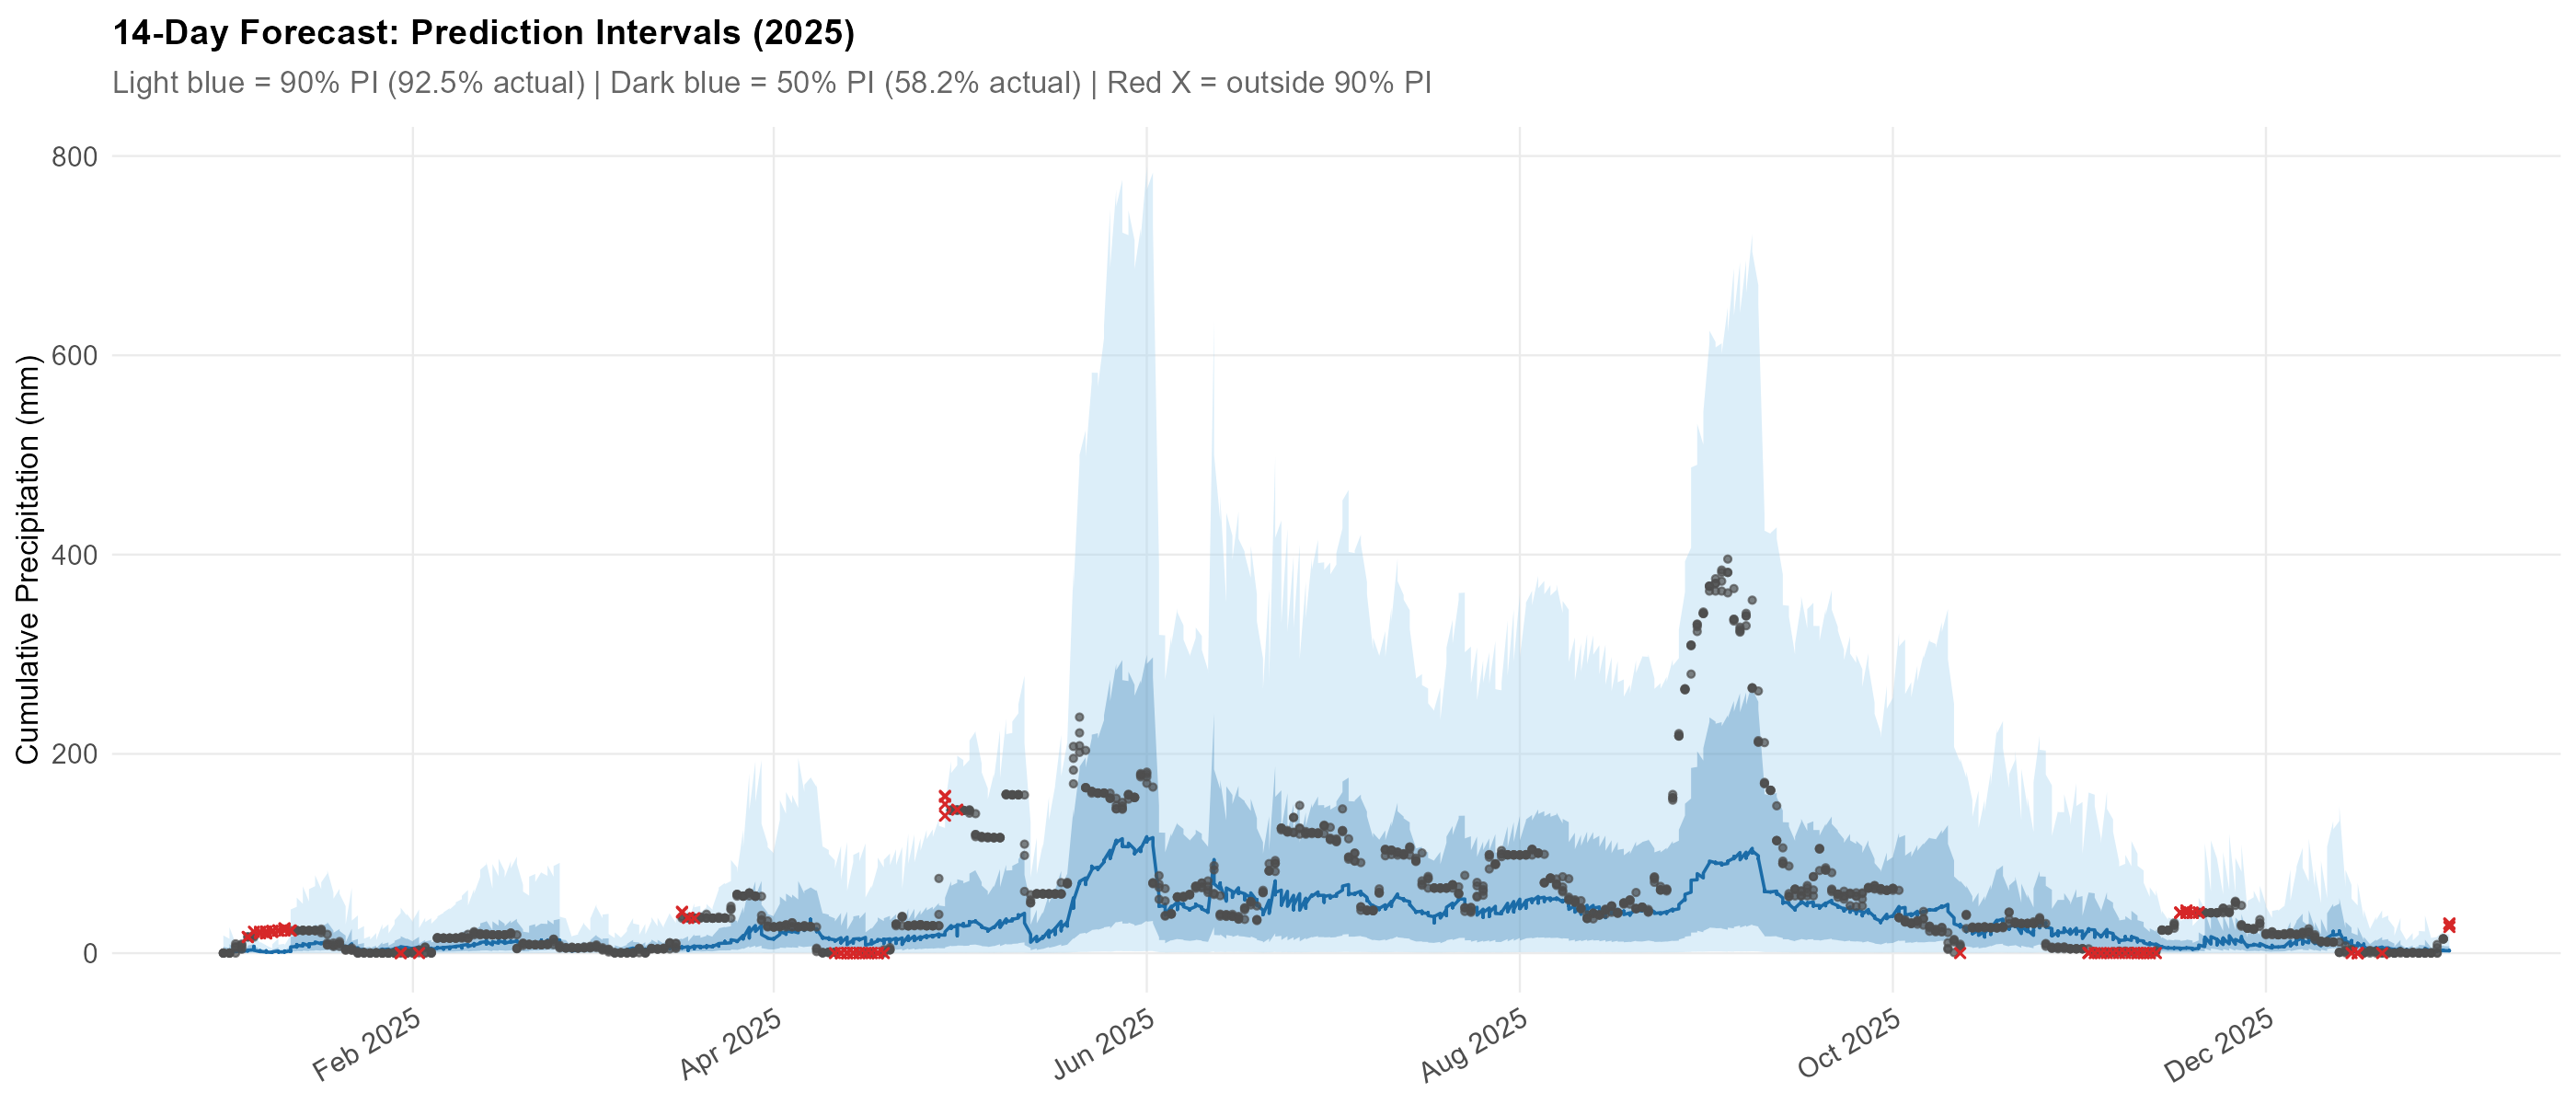
\includegraphics[width=\textwidth]{gamlss_14d_intervals.png}
    \caption{14-day cumulative precipitation forecasts for 2025. Light blue: 90\% prediction interval; dark blue: 50\% prediction interval; blue line: predicted median; black dots: observations within 90\% PI; red crosses: observations outside 90\% PI.}
    \label{fig:intervals}
\end{figure}

\subsection{Feature Importance}

Figure~\ref{fig:importance} shows the top 25 features by XGBoost gain. Climatology dominates at the 14-day horizon---\texttt{clim\_pct\_rainy} (what fraction of days are historically rainy for that time of year) is the top feature by a wide margin. Other climatological features like \texttt{clim\_iqr} and \texttt{clim\_p90} also rank high. This is not too surprising: at 14 days out, seasonal baselines carry a lot of information. That said, GEFS forecast features and bias correction features do show up in the top 25, so the NWP data is not useless---it just matters less than knowing what time of year it is.

\begin{figure}[H]
    \centering
    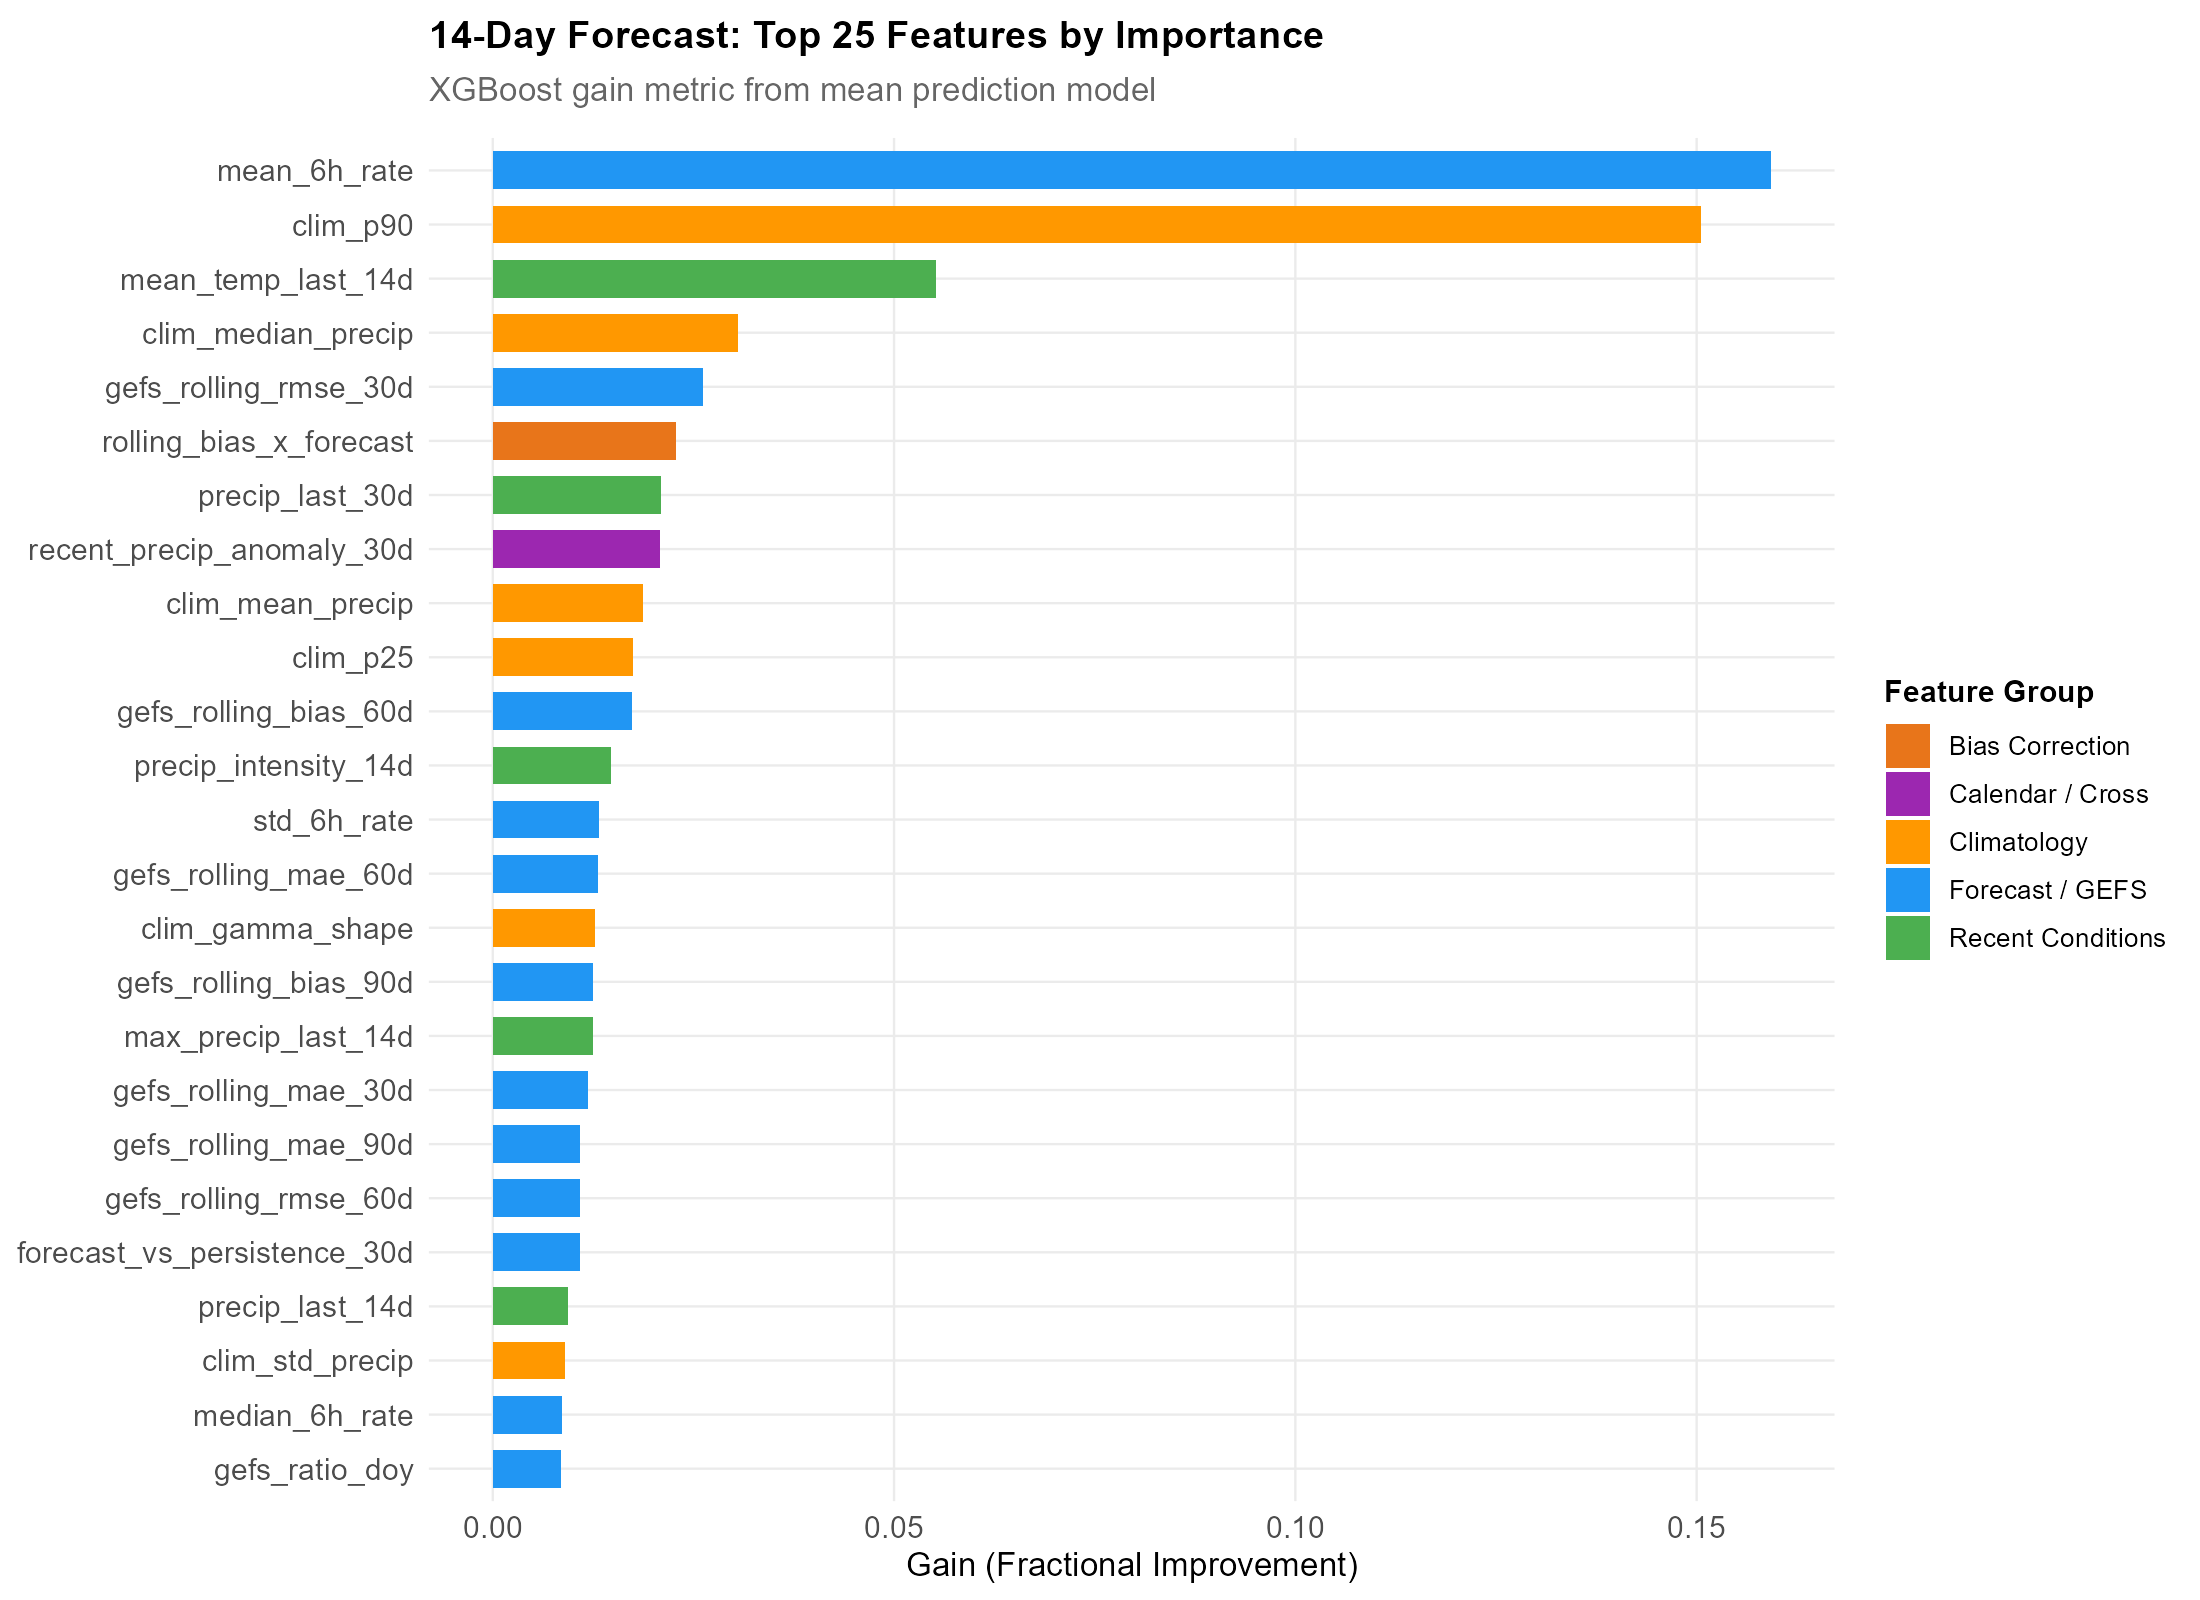
\includegraphics[width=\textwidth]{gamlss_14d_importance.png}
    \caption{Top 25 features by XGBoost gain for the 14-day mean model, colored by feature category.}
    \label{fig:importance}
\end{figure}

\subsection{Discussion}

The calibration here is a big improvement over our first attempt, where we used XGBoost's built-in \texttt{reg:gamma} objective and trained the variance model on squared residuals. That version only achieved 33\% actual coverage at the 90\% nominal level---basically the intervals were way too narrow. Switching to the log-transformed target, using absolute residuals with heavier regularization, and adding the post-hoc calibration step fixed most of this.

There are still issues. The Gamma distribution cannot put any probability mass at exactly zero, so the model struggles with dry periods---this shows up as a spike near zero in the PIT histogram. The validation set is also small (73 samples), which means the calibration factor we learn might not generalize perfectly to different years. For the final submission, we plan to train models at additional horizons (3, 7, 21, 28, 35 days) and look into zero-inflated distributions that can handle the dry days better.

% ─────────────────────────────────────────────────────────────────────────────
\bibliographystyle{plainnat}
\begin{thebibliography}{5}

\bibitem[Gneiting et~al.(2005)]{gneiting2005}
Tilmann Gneiting, Adrian~E. Raftery, Anton~H. Westveld, and Tom Goldman.
\newblock Calibrated probabilistic forecasting using ensemble model output statistics and minimum {CRPS} estimation.
\newblock \emph{Monthly Weather Review}, 133(5):1098--1118, 2005.

\bibitem[M{\"a}rz(2022)]{marz2022}
Alexander M{\"a}rz.
\newblock {XGBoostLSS}---An extension of {XGBoost} to probabilistic forecasting.
\newblock \emph{arXiv preprint arXiv:2204.06826}, 2022.

\bibitem[Rasp and Lerch(2018)]{rasp2018}
Stephan Rasp and Sebastian Lerch.
\newblock Neural networks for postprocessing ensemble weather forecasts.
\newblock \emph{Monthly Weather Review}, 146(11):3885--3900, 2018.

\bibitem[Schlosser et~al.(2019)]{schlosser2019}
Lisa Schlosser, Torsten Hothorn, Reto Stauffer, and Achim Zeileis.
\newblock Distributional regression forests for probabilistic precipitation forecasting in complex terrain.
\newblock \emph{Annals of Applied Statistics}, 13(3):1564--1589, 2019.

\bibitem[Taillardat et~al.(2016)]{taillardat2016}
Maxime Taillardat, Olivier Mestre, Micha{\"e}l Zamo, and Philippe Naveau.
\newblock Calibrated ensemble forecasts using quantile regression forests and ensemble model output statistics.
\newblock \emph{Monthly Weather Review}, 144(6):2375--2393, 2016.

\end{thebibliography}

\end{document}
